%%%%%%%%%%%%%%%%%%%%%%%%
%
% $Autor: Sudeshna Nanda $
% $Datum: 2024-12-03 $
% $Pfad: ML24-06-Magic-Wand-with-an-Arduino-Nano-33-BLE-Sense/report/Contents/en/Introduction.tex $
% $Version:### $
%
%%%%%%%%%%%%%%%%%%%%%%%%

\chapter{Introduction}

	The development of Machine Learning and the evolution of \ac{iot} have progressed hand-in-hand within these several years. The IoT Idea has permeated various aspects of our lives, such as healthcare, agriculture, intelligent cities, etc.\cite{Had:2020}. Also, lots of IoT applications should be able to process data to respond instantly. Handling such requirements by cloud computing is then not suitable\cite{shi:2016}.

	
	\ac{tinyml}, therefore, is a rapid enhancement in machine learning area due to its low-latency, low power and bandwidth model inference at edge devices\cite{sakr:2020}. TinyML primarily employs small form factor devices, for instance, \ac{RTOS} based microcontrollers, to run machine learning models and algorithms\cite{anh:2009}. Also, one of the most striking features of TinyML is its small size and, in some cases, its ability to function on battery power for years\cite{Aba:2023}. This technology heralds a new era of edge services and applications that are not reliant on cloud processing but rather thrive on distributed edge inference and autonomous reasoning.


	Arduino is one of the critical components of this project. It allows for the control of board behavior via instructions relayed to the board's microcontroller. Such instructions are provided using the Arduino \ac{ide}, based on Processing and the Arduino programming language. Arduino's original purpose was to serve as a simple prototyping tool for students without prior knowledge of electronics or programming. However, as the platform developed, Arduino boards began to diversify, expanding their scope from simple 8-bit boards to devices designed for IoT applications, wearable technology, 3D printing, and embedded environments\cite{kushner:2011}. This adaptability has enabled Arduino to meet new challenges and needs effectively. The Arduino IDE and its Programming Language allow for a high extent of customization to meet the user's requirements, making it a favored development platform for rapid prototyping and idea validation\cite{kushner:2011}.


	This paper delves into using the 3.3V board Arduino Nano 33 BLE Sense. The hardware features three-axis accelerometers, indicating its ability to detect motion and calculate acceleration in three dimensions\cite{Ard:2021}. The objective of this report is to construct a "Magic Wand" and integrate it with the board Arduino Nano 33 BLE Sense. The board is programmed to recognize predefined gestures, indicating movement direction for gesture recognition.
	
	
	The \ac{led} can be programmed to flash in response to hand movement commands in Arduino. When the wand is moved in a specified direction, the board interprets the gesture and converts it into a visual output. To create the magic wand, the board Arduino Nano 33 BLE Sense is attached to the end of a stick, and the accelerometer's data is fed into a deep-learning model to ascertain whether a recognized gesture has been made. The Arduino board's integral multi-dimensional detector is used to collect gestures, which are vital for understanding complex data. A model can be trained to understand and embed this complex data into the board Arduino Nano 33 BLE Sense.
	
	
	Additionally, \ac{tfl} is used to implement a Neural Network model to recognize gestures using an accelerometer. Triumphant gesture casting results in visualising the corresponding gesture on the screen and the Arduino board's LED lighting up in response to the human input.
	
	A heuristic function is integral to this application. It encodes gesture knowledge into code, requiring programming skills, mathematical knowledge, and domain expertise. The data collected from the accelerometer undergoes mathematical conversions to produce the desired output or the intended gestures. Instead of creating a heuristic method from scratch, users can select an appropriate model architecture, gather and label a dataset, and iteratively build a model through training and evaluation. The model uses the accelerometer data as input without pre-processing, performs inference, and analyses the results. Three movements have been trained: wing (w), ring (o), and slope (/). The direction of motion for the gestures is shown in the figures \ref{fig:Wing Gesture} \ref{fig:Ring Gesture} \ref{fig:Slope Gesture}. If the input is valid, it generates a visual output of the gestures on a terminal and responds to each spell by lighting an LED. There is also an output to denote an "unknown" gesture if any movement is not recognized.These "unknown" gestures are the motions which are not belong to the wing, ring and slope movements.
	
	\begin{figure}[H]\centering
		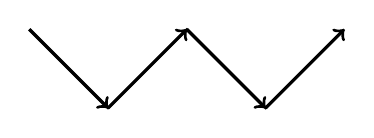
\begin{tikzpicture}
			% define point
			\coordinate (A)  at (1, 1);
			\coordinate (O)  at (2, 0);
			\coordinate (B)  at (3, 1);
			\coordinate (C)  at  (4,0);
			\coordinate (D) at  (5,1);
			% angle  
			\draw[thick] (A) -- (O) -- (B) -- (C)-- (D);
			%	\draw pic[draw=black,eccentricity=2.9]
			%\pic [draw,"$\alpha_1$",angle radius=20,->,angle eccentricity=1.4]
			%  {angle = B--O--A};
			\draw [->, very thick] (1,1) -- (2,0)  node [midway, above] {\scriptsize };
			\draw [->, very thick] (2,0) -- (3,1)  node [midway, above] {\scriptsize };
			\draw [->, very thick] (3,1) -- (4,0)  node [midway, above] {\scriptsize };
			\draw [->, very thick] (4,0) -- (5,1)  node [midway, above] {\scriptsize };
		\end{tikzpicture}
		\captionof{figure}{\textbf{Wing Gesture \cite{War:2020}}}
		\label{fig:Wing Gesture}
	\end{figure}
	
	\begin{figure}[H]\centering
		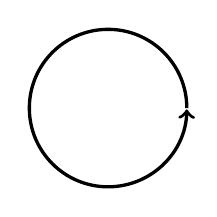
\begin{tikzpicture}
			\draw[->,very thick] (0,0) arc[radius=1cm,start angle=0,delta angle=359];
		\end{tikzpicture}
		\captionof{figure}{\textbf{Ring Gesture \cite{War:2020}}}
		\label{fig:Ring Gesture}
	\end{figure}
	
	\begin{figure}[H]\centering
		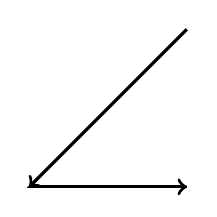
\begin{tikzpicture}
			% define point
			\coordinate (A)  at (2, 2);
			\coordinate (O)  at (0, 0);
			\coordinate (B)  at (2, 0);
			% angle  
			\draw[thick] (A) -- (O) -- (B);
			%\draw pic[draw=black,angle radius=20,angle eccentricity=1.4]
			%{angle = B--O--A};
			%\pic [draw,"$\alpha_1$",angle radius=20,->,angle eccentricity=1.4]
			%  {angle = B--O--A};
			\draw [->, very thick] (2,2) -- (0,0)  node [midway, above] {\scriptsize };
			\draw [->, very thick] (0,0) -- (2,0)  node [midway, above] {\scriptsize };
		\end{tikzpicture}
		\captionof{figure}{\textbf{Slope Gesture \cite{War:2020}}}
		\label{fig:Slope Gesture}
	\end{figure}
	
	The planning process encountered several challenges, including:
	
	\begin{itemize}	
		
		\item The size of the data model should be controlled at a reasonable level due to the limitation of memory in board Arduino Nano 33 BLE Sense \cite{shi:2016}
		\item Creating a Machine Learning data model for the four gestures, especially the "unknown" gesture
		\item The size of the data model should be controlled at a reasonable level due to the limitation of memory in board Arduino Nano 33 BLE Sense \cite{Ard:2021}
		\item Training the data model to get a more accurate result \cite{shi:2016}
		\item Avoiding extended waved gestures that could lead the accelerometer to record false readings and generate incorrect results.
		
	\end{itemize}


    \section{Problem's Description}

    Deploying deep learning (DL) models on edge devices like microcontroller units (MCUs) is a significant challenge due to their limited resources. Most DL algorithms are designed for high-performance systems such as GPUs or high-performance computing clusters, which makes them incompatible with the memory, computational, and energy constraints of MCUs. This poses a critical issue when adapting DL models for applications requiring real-time processing, such as industrial gauge inspection, where models must be optimized without losing significant accuracy or efficiency.
    
    \section{Challenges}
    
    \begin{itemize}
        \item \textbf{Resource Constraints:} \\
        Limited memory, computational power, and energy efficiency in MCUs restrict the deployment of traditional DL models. High-performance computer vision models exceed the capacity of edge devices.\cite{Ard:2021}
        
        \item \textbf{Accuracy vs. Efficiency Trade-off:} \\
        Reducing model size and computational complexity often results in performance degradation, particularly for computer vision tasks.\cite{shi:2016}
        
        \item \textbf{Framework Limitations:} \\
        Existing tools like TensorFlow Lite and AIfES offer optimization options but are not fully adapted to handle complex computer vision requirements on constrained hardware.\cite{Kristian:2020}
        
        \item \textbf{Real-world Application Needs:} \\
        Industrial applications, such as gauge inspection, require fast and accurate real-time image processing, which remains challenging to achieve on MCUs with existing models.\cite{Kristian:2020}
    \end{itemize}
    
    \section{Solutions}
    
    \begin{itemize}
        \item \textbf{Optimization Techniques:}
        \begin{itemize}
            \item \textbf{Quantization:} Convert weights and activations from 32-bit floating-point to lower-precision formats (e.g., 8-bit integers) to reduce memory and computation demands.
            \item \textbf{Pruning:} Eliminate redundant parameters in neural networks to reduce complexity without significantly affecting accuracy.
            \item \textbf{Knowledge Distillation:} Use large, pre-trained models to guide the training of smaller, more efficient models.\cite{Maciel:2023}
        \end{itemize}
        
        \item \textbf{Specialized Frameworks and Tools:}
        \begin{itemize}
            \item \textbf{TensorFlow Lite (TFLite):} Supports model optimization techniques like quantization and pruning and enables efficient execution on embedded devices.\cite{Kristian:2020}
            \item \textbf{AIfES:} Tailored for Arduino-based systems, allowing compact model creation and adaptation for 8-64 bit systems.
            \item \textbf{TinyNeuralNetwork:} Simplifies model compression and supports seamless integration between TensorFlow Lite and PyTorch.
            \item \textbf{CMSIS-NN:} Provides optimized neural network kernels specifically designed for ARM Cortex-M processors.\cite{Kristian:2020}
        \end{itemize}
        
        \item \textbf{Real-world Validation:} \\
        Implement and test optimized DL pipelines for tasks such as industrial gauge inspection, leveraging quantized and pruned models to meet performance and resource constraints. Use converted lightweight models for real-time processing tasks, ensuring that accuracy is maintained within acceptable thresholds.\cite{Kristian:2020}
    \end{itemize}
    
\section{Report Structure}
	Following the introduction, our report progresses to a comprehensive exploration of domain knowledge in second section. This section focuses on the nuances of data collection (\ref{chapter 2}), management, and its pivotal role, alongside an in-depth analysis of both the hardware (Arduino Nano 33 BLE Sense) in \ref{chapter 3} and the utilized software suite (Arduino IDE, TensorFlow, Python, etc.) in \ref{chapter 4} Subsequently, we delve into the utilization of \ac{cnn} in the realm of data mining in \ref{chapter 5}, elucidating their components and their pertinence to our project. The report then navigates through section 3, the intricacies of the \ac{kdd} Process (\ref{chapter 6}), covering its development (\ref{chapter 7}), deployment (\ref{chapter 8}), and the materials involved (\ref{chapter 9}). In section 4 conclusion, the report culminates by summarizing the principal discoveries and proposes avenues for future exploration and development.

